\begin{theo}[Kracht]{Kracht}

Een kracht is een actie die de snelheid van een voorwerp verandert. Elke versnelling wordt dus veroorzaakt door een kracht. Er zijn twee soorten krachten: 

\begin{itemize}
    \item \textbf{Contactkrachten:} fysisch contact vindt plaats
    \item \textbf{Veldkrachten:} werken op een zekere afstand
\end{itemize}

\hspace{-0.65cm} Een kracht is een vectoriële grootheid en heeft dus een grootte, richting en zin.

\end{theo}

\begin{lem}[De eerste wet van Newton: de Inertiewet]{De eerste wet van Newton: de Inertiewet}

Een lichaam in rust (of in eenparige rechtlijnige beweging) zal in rust (eenparige rechtlijnige beweging) blijven tenzij er een uitwendige resulterende kracht inwerkt

    \begin{equation*}
        \sum_{i} \Vec{F}_i = 0 \to \Vec{a} = 0
    \end{equation*}

\hspace{-0.65cm} Een \textbf{inertiaalstelsel} is een referentiestelsel waarin de eerste wet van Newton geldt. De \textbf{inertie} wordt gegeven door de massa en beschrijft hoeveel weerstand dat een lichaam biedt tegen een verandering van zijn snelheid. 

    % \begin{equation*}
    %     \dfrac{m_1}{m_2} = \dfrac{a_2}{a_1}
    % \end{equation*}

\end{lem}

\begin{lem}[De tweede wet van Newton: de versnellingswet]{De tweede wet van Newton: de versnellingswet}

De versnelling van een voorwerp is recht evenredig met de nettokracht op het voorwerp en omgekeerd evenredig met het massa van het voorwerp. De richting van de versnelling is dezelfde als de richting van de nettokracht.

    \begin{equation*}
        \sum_{i} \Vec{F}_i = \Vec{F}_{net} = m\Vec{a} = m\dfrac{d\Vec{v}}{dt} = m\dfrac{d^2\Vec{r}}{dt^2}
    \end{equation*}

\end{lem}

\begin{lem}[De derde wet van Newton: de actie-reactiewet]{De derde wet van Newton: de actie-reactiewet}

Wanneer een voorwerp een kracht uitoefent op een ander voorwerp, dan oefent het ander voorwerp een kracht met dezelfde grootte en omgekeerde zin uit op het voorwerp.

    \begin{align*}
        \Vec{F}_{1 \to 2} &= -\Vec{F}_{2 \to 1} \\
       F_{1 \to 2} &= F_{2 \to 1}
    \end{align*}

\end{lem}

\newpage

\begin{theo}[Gravitatiekracht]{Gravitatiekracht}
Alle voorwerpen nabij het aardoppervlak vallen met dezelfde versnelling $ \Vec{g} $. De kracht bepaald door deze vernselling wordt de \textbf{gravitatiekracht} of \textbf{zwaartekracht} genoemd:

    \begin{equation*}
        \Vec{F}_G = m\Vec{g}
    \end{equation*}

\noindent Deze kracht is gericht naar het aardoppervlak toe en de grootte wordt het \textbf{gewicht} van een voorwerp genoemd. 

\end{theo}

\begin{theo}[Normaalkracht]{Normaalkracht}
    De \textbf{loodrechte} kracht die het contactoppervlak uitoefent op het voorwerp 
    \begin{equation*}
        F_N = F_{g,y} - \sum_{rest,y} F_{rest,y}
    \end{equation*}
    \noindent wordt de normaalkracht genoemd. De volgende figuren tonen enkele veelvoorkomende situaties voor de oefeningen:
    
    \begin{minipage}{.48\textwidth}
    
        \centering
        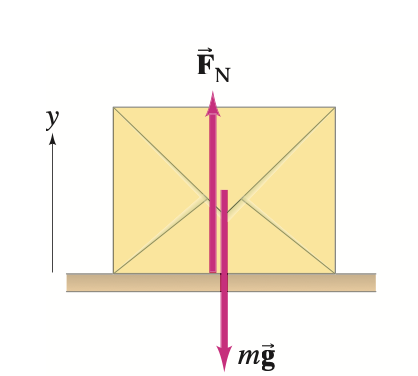
\includegraphics[scale = 0.7]{Images/Dynamica/Doos in rust.png}   
    
    \end{minipage} 
    \begin{minipage}{.48\textwidth}
    
        \centering
        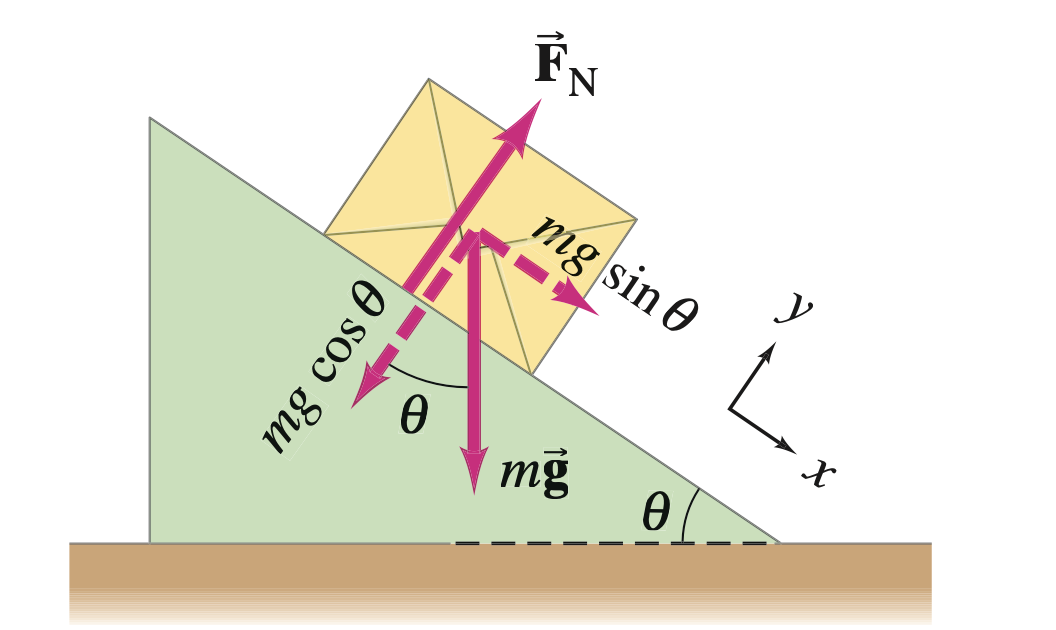
\includegraphics[scale = 0.35]{Images/Dynamica/Glijdende doos.png}
        
    \end{minipage}
    
    \vspace{0.25cm}
    
    \noindent De normaalkracht is dus afhankelijk van de gravitatiekracht van zijn grootte en zin, maar niet van zijn richting (zie de rechterfiguur). We kunnen dus \textbf{niet} zeggen dat het gravitatiekracht-normaalkracht paar een actie-reactie paar vormt. 
\end{theo}


